\begin{figure}
  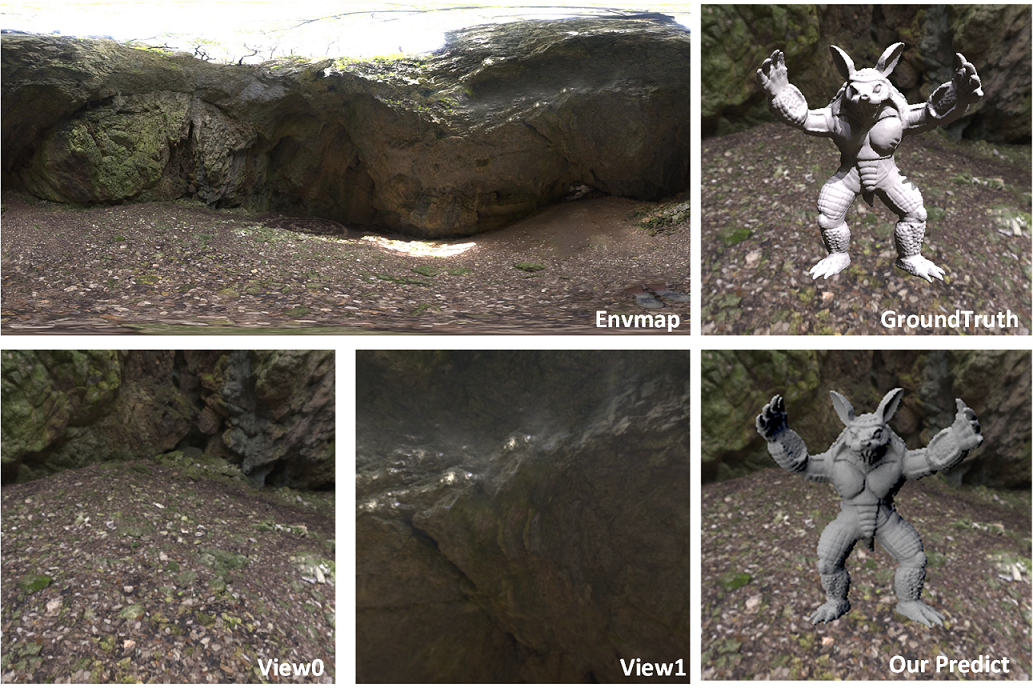
\includegraphics[width=\columnwidth]{Img/fig-failure.png}
  \caption[光照预测失败的例子]{
    \label{fig:failure-case}
    一种本文方法无效的情况。从图中可知全景图的顶部有一片十分强的光照区域,但是两幅输入图片都不包含推断这个光照的线索。此外这束强光属于该图中的高频信息,难以使用SH近似。由于这两个原因,在该图片上的预测结果与真实值相差甚远。}
\end{figure}